We begin by sketching the architecture of SDN networks and
describing the correctness challenges experienced by operators and
implementers of SDN control clusters.

SDN networks are managed by software running on a set of network-attached
servers called ``controllers''. Modern SDN platforms differ from
`first-generation' controllers such as NOX~\cite{nox} in two dimensions: they
extend vertically by providing a virtualization layer on top of which control
logic resides, and they extend horizontally by distributing state across
multiple control servers. We describe the correctness challenges imposed by
this complexity.

%Two common patterns of control are proactive and
%reactive. Proactive controllers pre-compute forwarding tables for the entire
%network, and only push down updates periodically to react to link failures,
%changes in traffic mix, \etc. In contrast, in \emph{reactive} SDNs, the
%controller updates the forwarding state in reaction to a \emph{dataplane event},
%e.g., a previously unmatched patched found on the wire.

%Production SDN deployments are commonly proactive, primarily due to the large
%scale of datacenter networks and the current capabilities of forwarding
%hardware. We focus on proactive controllers for the remainder of this paper,
%although our troubleshooting mechanisms are also applicable to reactive
%applications.

\subsection{Vertical Layering Challenges}

Modern SDN controllers consist of at least three distinct layers, as depicted in
Figure \ref{fig:basicarch}. The two lower layers are part of the SDN platform,
and the highest layer is the \emph{control application}. The lowest level of SDN
software maintains a graph data-structure known as the \emph{physical view}
that has a one-to-one correspondence with the physical network.
Synchronization logic in this layer keeps its information up-to-date with the
physical network state. Above, the \emph{Logical View} ideally translates the
potentially complicated physical network to into a simpler logical view, commonly a single
logical switch~\cite{Casado:2010:VNF:1921151.1921162}. This allows operators to
specify routing, access control, or QoS policies by configuring a single
forwarding device. If the control platform supports virtualization, a
virtualization layer handles multi-tenancy by providing each tenant with their
own logical view to specify policies over. The platform then multiplexes the
policies onto the same physical network.

At the top of the stack, the \emph{control application} specifies the desired
high-level behavior of the network. We term these behavioral specifications
``policies''. Policy constraints might include connectivity, access control,
addressing resource allocations, traffic engineering objectives, or middlebox
processing.

The logical view greatly simplifies the job of specifying policies. However, SDN
does not reduce the overall system complexity; it merely moves complexity out of
the control application and into the platform, which must transform these
high-level policy specifications into the appropriate configuration of each
physical device. When an entire datacenter network (up to 10,000 switches) is
abstracted into a single logical switch, the mapping between the logical switch
and the physical topology is highly complex.
%; for example, a simple configuration
%change such as ``the path from $A$ to $B$ should pass through $C$'' must be
%implemented as routing entries in a sequence of switches in the physical
%network. 

\eat{
This mapping is further complicated in a multi-tenant environment
\cite{Casado:2010:VNF:1921151.1921162} where each tenant specifies policies on
their own logical switch. In such a case, each controller must deal with
multiple tenants, and each tenant's policies must be coordinated among multiple
controllers. Maintaining isolation between tenants is critical; updates to the
physical network must therefore be performed in a consistent fashion to ensure
that isolation breaches do not occur for any in-flight packets, despite hardware
failures and message delays.
}

\subsection{Horizontal Layering Challenges}

For fault-tolerane, production SDN control software is typically \emph{physically
distributed} on several control servers. For scalability, the responsibility for
managing the network is partitioned hierarchically or through sharding between
several control servers. Onix~\cite{onix}, for example, partitions a
graph of the network state across either an eventually-consistent DHT or a
transactional database, allowing control applications to make their own
tradeoffs in choosing consistency models, degree of fault tolerance, and other
properties.

Policy changes that span multiple shards of the physical view
(statically-defined partitions of the physical network small enough to be managed
by a single control server) require coordination between controllers.
Coordination between controllers is prone to a plethora of well-known failure
modes, such as inconsistent reads, race conditions over message arrivals, and
unintended consequences of failover logic. Errors may also result from
non-disjoint partitioning schemes between controllers, or incorrect delegation
of control for different portions of the network.

\eat{
The large scale of these networks also means that
error events such as link failures or software crashes are common. Microsoft,
for example, reports 36M error events over one year across 8 datacenters, which
implies 8.5 error events per minute per
datacenter~\cite{Greenberg:2009:VSF:1592568.1592576}. 
}

\begin{figure}[t]
    %\hspace{-10pt}
    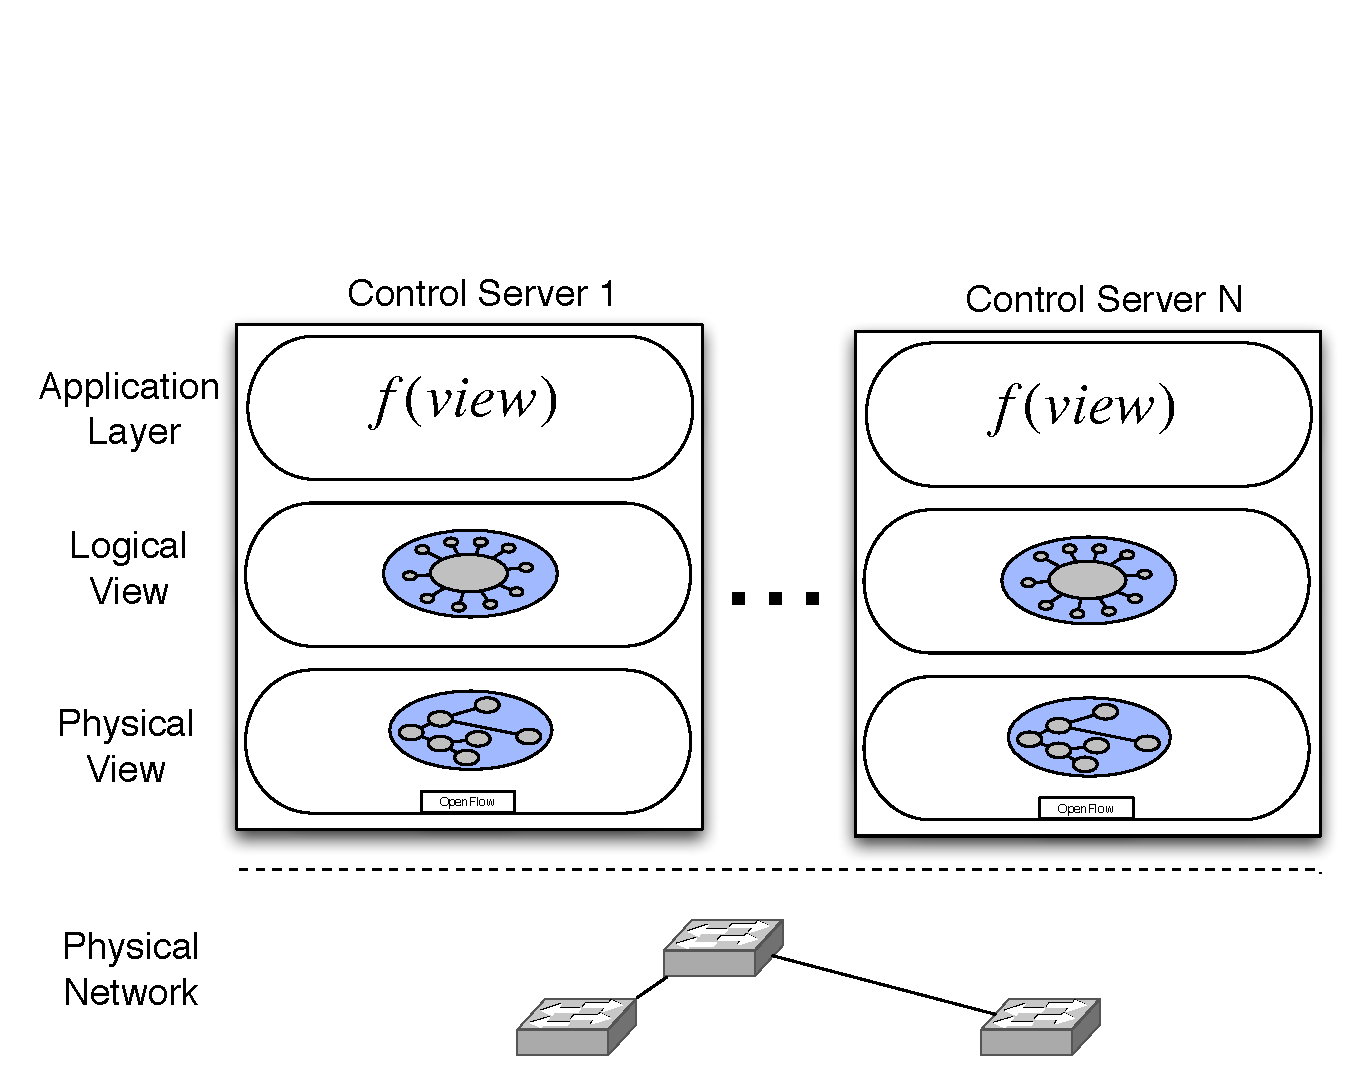
\includegraphics[width=3.25in]{../diagrams/architecture/SDN_Stack.pdf}
    \caption[]{\label{fig:basicarch} The SDN Software Architecture }
\end{figure}

In this paper we focus on bugs in the virtualization and controller coordination
components of the SDN software stack. We focus on a \emph{proactive} mode of
operation where forwarding state updates are triggered by policy or topology
changes, not data-plane events.\footnote{It seems feasible to generalize our
approach to include inputs from the data-plane.}
%We are primarily concerned with corner-case scenarios such as
%correlated hardware failures, which are the hardest to test {\it a priori}
%\andi{Check with our assuptions, i.e., uncorrelated external events}.
%Corner-case scenarios, while rare, cannot be ignored because of the distributed
%nature and large scale of production networks.
